% 固定来源第3页Q26：数学化重建上半支、抛物线、y=-x与PM。
% 选合法参数a=2作为绘图示例，m=(3+sqrt(5))/2，不添加到原题条件。
% P=(-2,2), A=(0,1), M=(0,m)，两条曲线严格满足题设焦点/过点关系。
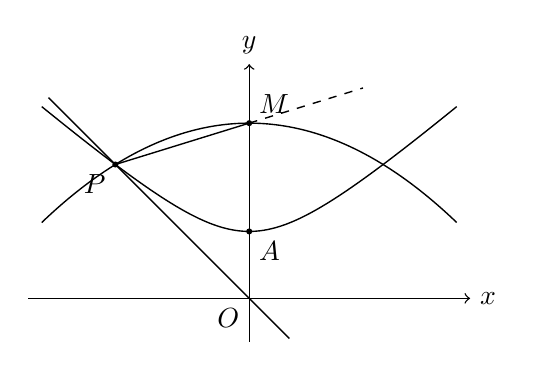
\begin{tikzpicture}[line width=.5pt,x=.85cm,y=.85cm]
  \pgfmathsetmacro{\vertex}{(3+sqrt(5))/2}
  \coordinate (O) at (0,0);
  \coordinate (A) at (0,1);
  \coordinate (P) at (-2,2);
  \coordinate (M) at (0,\vertex);
  \draw[->] (-3.3,0)--(3.3,0) node[right] {$x$};
  \draw[->] (0,-.65)--(0,3.5) node[above] {$y$};
  \draw[domain=-3.1:3.1,samples=100,smooth] plot (\x,{sqrt(1+.75*\x*\x)});
  \draw[domain=-3.1:3.1,samples=100,smooth] plot (\x,{\vertex-\x*\x/(4*(\vertex-1))});
  \draw (-3,3)--(.6,-.6);
  \draw (P)--(M);
  \draw[dashed] (M)--(1.7,{\vertex+1.7*(\vertex-2)/2});
  \fill (P) circle[radius=1.1pt] (A) circle[radius=1.1pt] (M) circle[radius=1.1pt];
  \node[below left] at (O) {$O$};
  \node[below right] at (A) {$A$};
  \node[below left] at (P) {$P$};
  \node[above right] at (M) {$M$};
\end{tikzpicture}
